
\documentclass[
	% -- opções da classe memoir --
	12pt,
	oneside,
	a4paper,
	english,
	brazil
	]{abntex2ppgsi}

% Pacotes básicos 

\usepackage[utf8]{inputenc}	
\usepackage{lastpage}	
\usepackage{indentfirst}
\usepackage{color}	
\usepackage{graphicx}	
\usepackage{microtype} 
\usepackage{pdfpages} 
\usepackage{algorithm}	
\usepackage{mdwlist}
\usepackage[noend]{algpseudocode}		
		
% Pacotes abnteX2
\usepackage{lipsum}	
\usepackage[brazilian,hyperpageref]{backref}
\usepackage[alf]{abntex2cite}
\renewcommand{\backrefpagesname}{Citado na(s) página(s):~}
\renewcommand{\backref}{}
% Define os textos da citação
\renewcommand*{\backrefalt}[4]{
	\ifcase #1 %
		Nenhuma citação no texto.%
	\or
		Citado na página #2.%
	\else
		Citado #1 vezes nas páginas #2.%
	\fi}%

\titulo{Em direção a um modelo de distribuição de vídeo sob demanda por meio de streaming adaptativo em redes CDN-P2P}

\autor{\uppercase{KAYRO FIGUEIRA PIRES}}
\local{Manaus}
\data{2016}
\orientador{Prof.Dr.: Cesar Augusto Viana Melo}

\tipotrabalho{Proposta de qualificação (Mestrado)}

\preambulo{
%\newline \newline \newline 
Proposta de qualificação apresentada ao Instituto de Computação da Universidade Federal do Amazonas, para qualificação no curso de Mestrado em Ciência da Computação pelo Programa de Pós-graduação em Informática.
%
\newline \newline Área de Computação: Redes de Computadores e telecomunicações}

% alterando o aspecto da cor azul
\definecolor{blue}{RGB}{41,5,195}

% informações do PDF
\makeatletter
\hypersetup{
     	%pagebackref=true,
		pdftitle={\@title}, 
		pdfauthor={\@author},
    	pdfsubject={\imprimirpreambulo},
	    pdfcreator={LaTeX com abnTeX2 adaptado para o PPgSI-EACH-USP},
		pdfkeywords={abnt}{latex}{abntex}{abntex2}{qualificação de mestrado}{dissertação de mestrado}{ppgsi}, 
		colorlinks=true,
    	linkcolor=blue,
    	citecolor=blue,
    	filecolor=magenta, 
		urlcolor=blue,
		bookmarksdepth=4 
        }
\makeatother
\setlength{\parindent}{1.25cm}
\setlength{\parskip}{0cm}  % tente também \onelineskip
\renewcommand{\baselinestretch}{1.5}
\makeindex
	% Controlar linhas orfas e viuvas
  \clubpenalty10000
  \widowpenalty10000
  \displaywidowpenalty10000

\begin{document}

\frenchspacing 
\imprimircapa
\setlength{\absparsep}{18pt}
\begin{resumo}
\end{resumo}

\chapter{Introdução}

Em 2019 o trafego de vídeo na Internet será 80\% de todo trafego consumido, sendo produzido aproximadamente um milhão de minutos de vídeo a cada segundo \cite{CISCO2015}. Nos últimos anos temos visto, ao longo da crescente popularidade dos vídeos na Internet, um aumento do tráfego servido por Redes de Distribuição de Conteúdo (CDNs - Content Delivery Network) [7],[8]. 
Esses tipos de redes replicam o conteúdo entre os seus servidores e os fornecem a usuários finais a partir do servidor mais próximo. CDNs distribuem grande parte do tráfego total da Internet: a estimativa varia de 15\% a 30\% de todo o tráfego da Web em todo o mundo para uma única popular CDN. 
CDNs tem problema de escalabilidade e custo, então para garantir o aumento/prevalência da distribuição de conteúdo multimídia, estudos apontam como solução escalável e de baixo custo o apoio de redes P2P na distribuição deste conteúdo [18].

Combinando as arquiteturas CDN e P2P em um sistema híbrido; teórica e praticamente tem se mostrado como um sistema factível, menos custoso e escalável. Segundo[15], é possível com o uso de redes P2P em apoio a CDNs na distribuição de conteúdo, uma redução de carga de 30\%-40\% sobre o servidor da CDN na distribuição de conteúdo moderadamente popular.
Por si só essas novas arquiteturas não resolvem de maneira ótima os problemas na distribuição de conteúdo, segundo \cite{Kangasharju2007}, dada a natureza intermitente da conexão dos pares nas largas comunidades P2P, é necessário considerar o gerenciamento de conteúdo na replicação e substituição de arquivos para alcançar performance satisfatória.

Uma das propostas largamente adotadas por provedores de conteúdo é o streaming adaptativo,em que cada arquivo de vídeo no servidor é codificado em J versões a decrescentes taxas de bits, e cada versão é dividida em H segmentos \cite{Tian2013}, portanto, quando um cliente solicita um vídeo ao servidor, este precisa escalonar os hj-ézimos segmentos que melhor se adaptam as condições de transmissão da rede, as quais, variam em função do tempo, mantendo assim a continuidade do fluxo de transmissão.

Dessa forma, torna-se importante o estudo de soluções que considerem o streaming adaptativo em redes P2P que apoiam CDNs na distribuição de conteúdo multimídia.

\section{Descrição do Problema}
 
A Internet praticamente dobra a cada dois anos e meio em tamanho e escala e o serviço mais proeminente nesta, é o tráfego de vídeos, que representa 66\% do tráfego de dados,de modo que ,dificuldades em minimizar a carga sobre o servidor e melhorar a qualidade de vídeos distribuídos por meio de streaming adaptativo em redes P2P que apoiam CDNs, é uma realidade enfrentada por pesquisadores da área de computação,  como desenvolver e operar estes serviços visando melhorar a qualidade de vídeos nas redes P2P, sem comprometer o fluxo da rede e reduzir a carga sobre o servidor?

\section{Motivação}

Relatórios indicam que o Netflix, uma aplicação de distribuição de vídeo sob-demanda, nos Estados Unidos é a aplicação que domina o tráfego nas infraestruturas de rede cabeadas. [22]. O YouTube, também uma aplicação de distribuição de vídeo sob-demanda, cujo conteúdo é produzido por seus usuários e de acesso gratuito, é a segunda aplicação em geração de tráfego nas redes cabeadas da Europa. Na Ásia o YouTube é a aplicação que mais gera tráfego nas infra-estruturas.[23]
Os mashups são aplicações da Web 2.0 formadas a partir da composição de recursos da própria Web [25](Ex: Facebook) , também contribuem para a proliferação de conteúdo multimídia. Até 2016 os vídeos representarão 66\% do tráfego de dados na internet segundo[19].
Para satisfazer a demanda de tais serviços, redes de distribuição de conteúdo (CDNs) são projetadas sobre as infraestruturas de telecomunicações, contudo devido ao enorme custo dos equipamentos para armazenamento e distribuição desse conteúdo, tem sido dada renovada atenção das indústrias de tecnologias de informação e comunicação(TICs) para estudos no desenvolvimento e operação destas redes que busquem incluir maior eficiência na distribuição desse tipo de conteúdo com o apoio de redes P2P.
A motivação desta proposta de trabalho é investigar  um modelo de distribuição de vídeo sob demanda por meio de streaming adaptativo em redes CDN-P2P que minimize o custo sobre o servidor e melhore a qualidade de vídeo em termos de bits recebidos no conteúdo compartilhado em redes P2P que apoiam CDNs na distribuição deste conteúdo.


\section{Justificativa}


\section{Objetivo Geral}

Propor e avaliar políticas de escalonamento de segmentos integradas a uma técnica de gerenciamento de buffer em redes P2P, considerando a distribuição de vídeos sob demanda por meio de streaming adaptativo que reduza a carga de trabalho do servidor, mantenha o fluxo da rede e ofereça maior qualidade em termos de bits recebidos para os vídeos baixados pelo usuário.


\section{Objetivos específicos}

Os objetivos específicos que direcionam este trabalho são:

\begin{itemize}
\item	Identificar o estado da arte no uso do streaming adaptativo na distribuição de conteúdo multimídia na internet.
\item 	Propor melhorias nas técnicas identificadas e definir ferramentas e metodologias para desenvolvimento do trabalho;
\item 	Experimentar em um estudo de caso, por meio de um simulador, um modelo de distribuição de conteúdo por meio de streaming adaptativo que minimize o custo de transmissão sobre o servidor e melhore a qualidade em termos de bits recebidos nos vídeos compartilhados em redes CDN-P2P;
\item 	Avaliar o modelo proposto analisando numericamente os custos sobre o servidor e a melhoria na qualidade do conteúdo de vídeo, comparando com modelos que representam o estado da arte na distribuição de conteúdo com o uso de streaming adaptativo em redes P2P que apoiam CDNs;
\end{itemize}

\section{Organização do Trabalho}

O primeiro Capítulo apresenta o cenário de streaming adaptativo na distribuição conteúdo multimídia, os conceitos iniciais sobre CDNs,streaming adaptativo, os problemas enfrentados em conter os crescentes custos no armazenamento e distribuição de conteúdo diante da crescente popularidade dos vídeos
O Capítulo 2 apresenta os fundamentos teóricos e os conceitos sobre distribuição de vídeos sob demanda,arquitetura de redes de distribuição de conteúdo e streaming adaptativo na distribuição de conteúdo em redes CDN-P2P.
O Capítulo 3 apresenta os trabalhos relacionados mais relevantes sobre as definições, modelos, técnicas e estratégias relacionados ao tema que está sendo abordado. 
O Capítulo 4 descreve o modelo proposto, por meio de uma arquitetura implementada em ambiente simulado para condução dos experimentos , apresentando em ordem sequencial como o mesmo será desenvolvido e posteriormente analisado numericamente.
O Capítulo 5 apresenta as considerações deste trabalho, onde serão descritas as dificuldades encontradas, as sugestões para trabalhos futuros e contribuições da pesquisa para a ciência bem como para a sociedade. Ao final, são apresentadas as conclusões deste trabalho relacionando desde o objetivo até sua conclusão com a análise dos resultados numéricos.



\chapter{Fundamentos Téoricos}

\section{Vídeo sob Demanda}

 

\section{Arquitetura Híbrida CDN-P2P}






\section{Principais Métodos de transmissão de vídeo}

Os principais métodos de distribuição de vídeo são três: streaming tradicional, download progressivo e streaming adaptativo. No streaming tradicional o arquivo  é dividido em pedaços menores e sua reprodução é individual e contínua a medida que cada pedaço é baixado. No download progressivo o vídeo é dividido em segmentos e ao longo de toda a  sessão  apenas uma taxa de bits é selecionada, os segmentos são armazenados no cliente dando vazão ao conteúdo, com a piora das condições da rede podem ocorrer interrupções e congelamentos na reprodução do vídeo.

No streaming adaptativo o vídeo é codificado a diferentes taxas de bits  criando diferentes versões desse vídeo, com o mesmo tempo de playback, cada versão é dividida em segmentos de mesma duração. Chama-se representação o conjunto de características do versionamento de um vídeo, tais como, o número de versões, a quantidade, o tamanho e duração dos segmentos. Nesta abordagem a transmissão é contínua e o conteúdo é descartado após ser apresentado, mas a característica fundamental é adaptar a taxa de bits do vídeo ao longo da sessão de acordo com as variações das condições da rede . Fatores como largura de banda, vazão e buffer são avaliados para um melhor ajuste da taxa de bits, proporcionando continuidade ao fluxo de vídeo e uma melhor experiência de visualização ao usuario.(SEUFERT et al., 2013).

\section{Streaming adaptativo}
No streaming adaptativo cada arquivo de vídeo é dividido em J versões e cada versão é dividida em H segmentos e todas as versões tem o mesmo tempo de playback X (Tian et al., 2013), Chama-se representação o conjunto de características do versionamento de um vídeo, tais como, o número de versões, a quantidade, tamanho e duração dos segmentos.

\begin{figure}[H]% H manda colocar exatamente nessa posição no texto (relativa aos parágrafos anterior e posterior)
	\centering
 	  \caption{Representação de um vídeo para streaming adaptativo}
		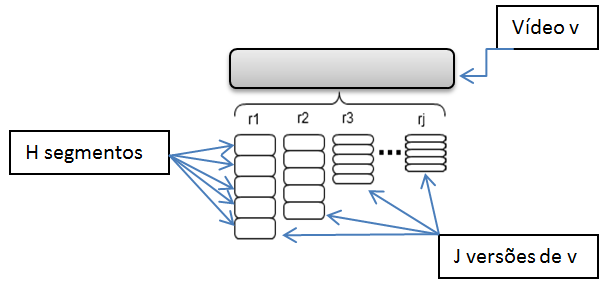
\includegraphics{figuras/segmentos.png}
	%\label{figura1:Streaming adaptativo em uma rede P2P}
  \source{Autor, 2016}
\end{figure}



\chapter{Trabalhos Relacionados}

Neste capítulo apresenta-se os trabalhos que tratam dos métodos de distribuição de vídeos sob demanda por meio de streaming adaptativo em redes P2P,as redes P2P revolucionaram o compartilhamento de conteúdo na ultima década, mas que ainda não são largamente exploradas comercialmente. as redes Híbridas CDN-P2P, são apontadas como soluções factíveis e menos custosas em relação a distribuição de conteúdo, aborda-se o atual uso do streaming adaptativo dinâmico nestes cenários, bem como, as políticas de gerenciamento de conteúdo e conclui-se com as considerações finais sobre o capítulo.

\section{Distribuição de vídeo sob demanda}
\subsection{Em redes P2P}

Em \cite{Kangasharju2007}, apresenta-se um modelo para controle de replicação em uma rede P2P formada em torno de uma comunidade que compartilha interesses e é atendida pelo mesmo provedor de acesso. Considerando replicação, políticas de substituição de arquivos e balanceamento de carga para o aumento da disponibilidade de conteúdo e da taxa de acerto intra-comunidade. A popularidade dos arquivos segue uma distribuição Zipf-like, o gerenciamento de conteúdo é feito por um algoritmo chamado Top-K mais frequentemente requisitado e aborda-se o balanceamento de carga por meio da fragmentação de arquivos e de uma técnica de overflow.Com remoção da restrição de integralidade, cria-se um limite superior para o modelo de otimização que maximiza a taxa de acerto,formula-se a replicação ótima chamada, "Logarithmic Replication Rule".Por meio de simulação avalia-se os algoritmos propostos, conclui-se que o algoritmo Top-k mais frequentemente requisitado quase sempre alcança performance ótima.A fragmentação de arquivos melhora a distribuição do conteúdo, mas pode ser ajustada com a abordagem overflow.


No trabalho de \cite{Tian2013} é apresentada uma proposta de streaming dinâmico para redes P2P com mecanismos de incentivo baseados em teorias de jogos cooperativos, neste cenário há um swarm para cada uma das diferentes versões de um vídeo,onde, pares que contribuem com mais recursos, podem ser recompensados recebendo versões de alta qualidade.Pares assistindo a mesma versão compartilham chunks de vídeo uns com os outros, reduzindo os custos de banda sobre o servidor. Desenvolve e simula-se um algoritmo distribuido de streaming dinâmico para comunidades formadas por pares que compartilham o custo de um conteúdo pago e também para comunidades que compartilham conteúdo gratuito. Conclui-se que o sucesso do streaming dinâmico em redes P2P tem como ponto principal os mecanismos de incentivo. Por meio de simulação demonstra-se a eficiência dos mecanismos de incentivo e do algoritmo de streaming dinâmico.

No trabalho de \cite{Xu2013}é apresentada uma análise do potencial uso do streaming adaptativo, tal como o DASH ( Dynamic Adaptive Streaming over HTTP ) em redes P2P, avalia-se a performance do streaming adaptativo em redes P2P em face das variações de banda e churn dos pares. Por meio de análise e simulação apontam que o uso do streaming adaptativo em redes P2P não só reduz a carga sobre o servidor, mas melhora a percepção do usuário sobre a qualidade do vídeo diante das dinâmicas variações de banda.

\subsection{ em redes híbridas CDN-P2P}
Em \cite{Zhang2015} É realizado o estudo de um serviço de vídeos sob demanda sobre uma rede híbrida CDN-P2P.Localizado na China, o provedor de serviços Kankan adota uma rede híbrida fracamente acoplada, implanta uma escala CDN em três clusters geográficos, adota um mecanismo para melhorar o delay inicial do straming de vídeo.

Coletou-se os ID's dos vídeos e IP's dos servidores por meio de uma rede P2P de rastreadores, foram enviadas solicitações de vídeos aos servidores usando os dados coletados, de modo que, as respostas com as listas dos pares candidatos a fornecer os vídeos, eram gravadas para posterior análise. Observou-se que haviam mais de 3 milhões de clientes ativos diariamente, e que o conteúdo nos caches dos pares muda muito lentamente e que por isso reduzem eficientemente o número de requisições ao servidor comparadas com servidores sem apoio de uma rede P2P.
Conclui-se que a rede P2P contribui com 98\% do conteúdo de vídeo mais popular e que em geral o mecanismo dual-server melhora o delay inicial do streaming de vídeo. Kankan formece um serviço de streaming de VoD em grande escala sobre infra-estrutura fixa de pequena escala, devido a lenta variação de conteúdo nos caches dos pares, somada a mecanismos de aprimoramento na CDN.




%Ge Zhang, Wei Liu, Member, IEEE, Xiaojun Hei, Member, IEEE, and Wenqing Cheng,

\section{Políticas de Gerenciamento de conteúdo}

Em \cite{Oliveira} os autores apresentam políticas de gerenciamento de objetos para melhorar a disponibilidade de conteúdo em sistemas CDN-P2P. Quatro políticas são propostas e avaliadas usando simulação com modelos de dados de coleções de vídeos do youtube. Em alguns casos as políticas propostas foram capazes de melhorar em mais de 70\% a disponibilidade de conteúdo comparada a disponibilidade proporcionada pela política LFU e mais de 50\% comparada a política GDSP.

Em \cite{Kangasharju2002}estuda-se o problema de replicação de objetos em servidores de uma rede CDN. de modo que,o objetos possam ser servidos por um servidor mais próximo ao cliente que o requisita. Mostra-se que o problema é NP-Completo e o formulam como um problema de otimização combinatória,buscando minimizar o número de servidores,esta análise  é feita sobre uma parte da topologia real da internet.
Mostram a comparação entre 4 heurísticas de replicação de objetos, RANDOM, POPULARITY, GREEDY-SINGLE, GREEDY-GLOBAL.
Conclui-se que a melhor performance é da heurística Greedy-Global na qual todos os servidores CDN cooperam nas decisões de replicação, distando 24\% da heurística mais simples.
O trabalho também aponta em direção a um modelo de distribuição de conteúdo em redes par-a-par, que estuda os benefícios de cooperação entre os nós, e mostram que os nós usando uma simples heurística e cooperação inteligente podem obter ganhos de performance significativos.


\section{Considerações do Capitulo}

Os trabalhos correlatos aqui apresentados deixam algumas lacunas deste cenário de redes de distribuição de conteúdo multimídia, que considere melhora na qualidade do conteúdo de vídeo, em comunidades P2P que apoiam CDNs na distribuição de vídeos sob demanda por meio de streaming adaptativo. Segundo os próprios autores podem ser explorados em trabalhos futuros, dessa maneira,pretende-se ao final deste trabalho, apresentar um modelo de distribuição de conteúdo que minimizem o custo sobre o servidor na distribuição de conteúdo multimídia em redes CDN-P2P, considerando melhor qualidade de vídeo em termos de bits recebidos no download ou substituição de vídeos nos pares de redes P2P.

\chapter{Controle de Replicação em uma CDN-P2P que distribui Vídeo ABR}

%\newcommand{\vetu}{$u_i=(u_1,u_2,\ldots,u_n)$}
Neste capítulo a replicação controlada de conteúdo é caracterizada como um problema de programação linear Inteira. A replicação ocorre em uma rede CDN-P2P dedicada a distribuição de vídeos com taxas de consumo adaptável as condições de rede. Os $N$ pares que participam do swarming $P$, formado em torno da distribuição do vídeo $v$, aceitam compartilhar segmentos de $v$ replicados de forma pró ativa e sob sua posse até um volume $s$.

O vídeo $v$ é versionado com diferentes taxas de bits $(r_1,r_2,\ldots,r_J)$, i.e. qualidades, e cada versão é segmentada e alinhada no tempo, gerando $H$ segmentos de duração $t$ por versão e permitindo que os pares acessem, segmentos de qualidade distintas. As informações de todas as versões de $v$ encontram-se em uma playlist $Z$, repassada ao par $i$ quando este se junta ao swarming. Usando as informações em $Z$, um algoritmo de seleção deve escolher, em um determinado instante $t$, qual é a qualidade do próximo segmento a ser baixado. Essa decisão deve considerar:
\begin{itemize}
\item os recursos de transmissão disponível;
\item a continuidade da sessão de vídeo;
\item a qualidade do segmento acessado;
\end{itemize} 

O recurso de transmissão de um par $i$ é limitado e definido por suas taxas de upload $u_i$ e download $d_i$. Em outras palavras, ao atuar como servidor no swarming, o par $i$ estará limitado no atendimento pela suas taxa de upload $u_i$. E ao atuar como cliente, ele estará limitado por sua taxa de download $d_i$.

A continuidade da sessão de acesso é impactada pela disponibilidade dos segmentos que têm tempo de reprodução definido na k-ésima janela de tempo $w_i(k)$. Um mecanismo de janela deslizante é usado para definir $w_i(k)$:

\begin{equation}
w_i(k) = \frac{d_i\bar{D}_i(k-1)}{\bar{L}_i(k-1)} 
\end{equation}

\noindent $d_i$ é o atraso inicial da reprodução para o par $i$, e, para as últimas $k-1$ janelas, $\bar{D}_i(.)$ e $\bar{L}_i(.)$ são respectivamente a taxa média de consumo do vídeo e tamanho médio dos segmentos acessados.

O algoritmo de escalonamento deve baixar os próximos segmentos com tempo de reprodução definido na janela $w_i(.)$, objetivando sempre os segmentos com maior taxa de bits, de forma a garantir a qualidade do fluxo.  A Figura \ref{fig:StreamingAdaptativo} mostra os elementos e a dinâmica descrita anteriormente.

\begin{figure}[H]% H manda colocar exatamente nessa posição no texto (relativa aos parágrafos anterior e posterior)
	\centering
	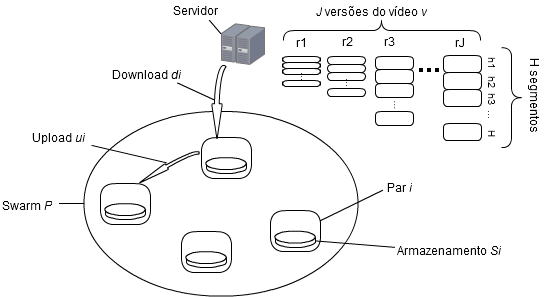
\includegraphics[height=5cm,width=0.8\textwidth]{figuras/Streaming_swarm.png}
 	 \caption{Streaming adaptativo em uma rede P2P}
	\label{fig:StreamingAdaptativo}
  %\source{Autor, 2016}
\end{figure}

 O problema modelado a seguir considera as seguintes variáveis do problema:


\begin{description}
\item[N] 	é o número de pares no swarming.
\item[H] 	é o número de segmentos do vídeo. 
\item[T] 	é o tempo de playback do vídeo $v$.
\item[t] 	é o tempo de duração dos segmentos do vídeo $v$.
\item[$u_i$] é a capacidade de upload do par i.
\item[$u_s$] é a capacidade de upload do servidor.
\item[d] 	é a capacidade de download do par i.
\item[X] 	é tempo de latência antes da visualização do objeto.
\item[$h_j$] 	é o h-ésimo segmento na versão \textit{j} do filme \textit{v}  ,todo segmento na versão $j$ tem o mesmo tamanho e duração.
\item[L] 	é o tamanho do vídeo.
\item[$l_{vj}$] 	é a duração do segmento de vídeo.
\item[$S_i$] 	é a capacidade de armazenamento par $i$.
\item[S] 	é a capacidade de armazenamento total do swarm.
\item[W] 	tamanho da janela de tempo para download de $M$ segmentos.
\item[b]  	é a taxa de visualização.
\item[J]  	é o número de versões na playlist.
\item[P]  	é um swarm ( conjunto de pares ).
\item [Z]	é a playlist com J versões.
\item[$B_h$]	é o tamanho em bytes dos $h$ segmentos.
\end{description}



\section{Modelo de Otimização}


\newcommand{\veth}{$h_{j}=(h_{1j},h_{2j},h_{3j},\ldots,H_j)$}


O vídeo $v$ possui $J$ versões e cada versão $j$ é dividida em $H$ segmentos, e que $M$ segmentos garantem uma continuidade da sessão de acesso em um nível ótimo. O tamanho de cada segmento $l_j$ é determinado por $l_j$=$L_j$/$H$, onde $L_j$ é o tamanho do vídeo na versão $j$.
% * <cavmelo@icomp.ufam.edu.br> 2016-03-26T09:43:35.819Z:
%
% > e que determinado $M$ de segmentos são necessários para reconstruir o vídeo
%
% Qual a razão dessa diferença entre H e M? 
%
% ^.
Sobre esta análise, assume-se que os pares estão ativos na comunidade com probabilidade homogênea, $p_i=p$ para todos os pares.
Nos referimos ao h-ésimo segmento da versão $j$ como \veth. Para uma atribuição fixa de cópias aos pares. Dado $B_h$ ser o tamanho em bytes das réplicas dos $h_j$ segmentos armazenados na comunidade, Temos:

% Dado $n_{hj}$ ser o número de réplicas do segmento $h_j$ armazenados na comunidade e $B_h$ ser o tamanho em bytes de  $n_{hj}$, Temos:
\begin{equation}
Max  \ \ B_h=\sum_{j=1}^{J}\sum_{h=1}^{H}l_{jh}
\end{equation}

Sujeito \ a:
\begin{equation}
\sum_{i=1}^{I}\sum_{j=1}^{J}\sum_{h=1}^{H}x_{ijh}l_{jh} \leq S,
\end{equation}
\begin{equation}
\sum_{i=1}^{I}\sum_{j=1}^{J}x_{ijh} \leq 1 ,\ h = 1, \dots, H
\end{equation}

\begin{equation}
\sum_{j=1}^J\sum_{h=1}^{H}x_{ijh}\frac{l_{jh}}{U_i} \leq W_i ,i = 1, \dots, I
\end{equation}

O tamanho da janela de tempo W é igual ao tempo de latência X necessário para preencher o buffer, nesta janela devem contem os m segmentos necessários para manter o fluxo no tempo de playback
\begin{equation}
W = X
\end{equation}

% \begin{equation}
%   \sum_{j=1}^{J}\sum_{h=1}^{H}\frac{Lj}{M}n_{jh}\leq S
% 	\label{eq:equacao-exemplo4}
% \end{equation}


% \section{Representação de um vídeo para streaming adaptativo}

% No streaming adaptativo cada arquivo de vídeo é dividido em J versões e cada versão é dividida em H segmentos e todas as versões tem o mesmo tempo de playback X (Tian et al., 2013), 
% Chama-se representação o conjunto de características do versionamento de um vídeo, tais como, o número de versões, a quantidade, tamanho e duração dos segmentos.


% \begin{figure}[H]% H manda colocar exatamente nessa posição no texto (relativa aos parágrafos anterior e posterior)
% 	\centering
%  	  \caption{Representação de um vídeo para streaming adaptativo}
% 		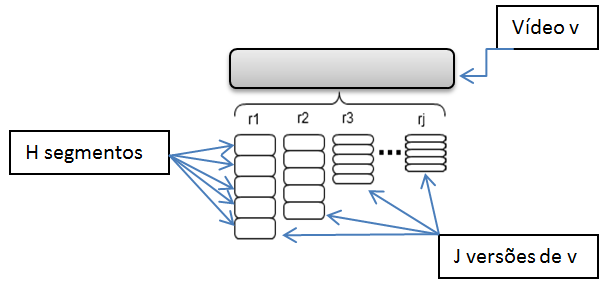
\includegraphics{figuras/segmentos.png}
% 	%\label{figura1:Streaming adaptativo em uma rede P2P}
%   \source{Autor, 2016}
% \end{figure}

% O tracker identifica e mantem uma lista dos pares e seus recursos que entram no swarm, como banda de upload/download e capacidade de buffer, então fornece uma lista de pares possíveis para conexão, o qual, é capaz de consumir e compartilhar segmentos de vídeo.
% Número de versões ideal (Xu et al., 2013)
% Para escalonamento de download dos segmentos, pretende-se usar uma política greedy, priorizando segmentos com maior qualidade em termos de bits recebidos.



\section{Políticas de escalonamento para downloads de segmentos.}

Para escalonamento de download dos segmentos, pretende-se usar uma política greedy, priorizando segmentos com maior qualidade em termos de bits recebidos.
O objetivo é maximizar a quantidade de segmentos de maior qualidade entre os pares, para isso considera-se a taxa de bits, tamanho e duração do segmento. Quanto ao par, consideramos a capacidade de armazenamento, banda de upload e download . Cada par mantém uma janela deslizante de tempo com segmentos para fazer o download, avançando a medida que o vídeo é reproduzido (Tian et al., 2013), portanto, é necessário escalonar dentro dessa janela de tempo, quais segmentos e suas respectivas taxas $j$ do vídeo $v$ serão baixados, de maneira que mantenha a maior qualidade, sem comprometer o fluxo de reprodução, a figura 2 ilustra esse cenário( construir a figura ).

\begin{figure}[H]% H manda colocar exatamente nessa posição no texto (relativa aos parágrafos anterior e posterior)
	\centering
 	  \caption{Problema de decisão sobre que segmentos e respectivas taxas j do vídeo v serão baixadas.}
		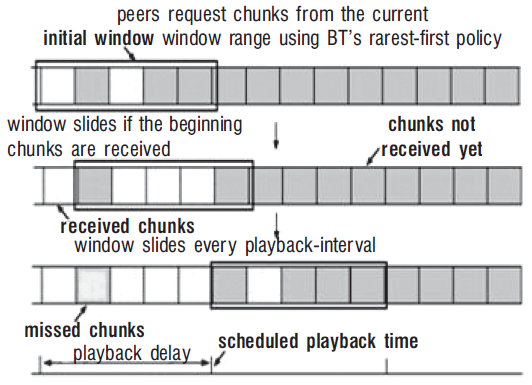
\includegraphics{figuras/janeladetempo.png}
	%\label{figura1:Streaming adaptativo em uma rede P2P}
  \source{Autor, 2016}
\end{figure}

Uma janela deslizante de tempo é o intervalo de tempo $W=bd/l$, onde $b$ é a taxa de visualização, $d$ é a taxa de download e $l$ é o tamanho do segmento. A taxa de download deve ser no mínimo igual a taxa de transmissão do objeto, para que o par tenha capacidade consumir a respectiva taxa produzida; esta janela possui os próximos $h$ segmentos a serem baixados e avança a medida que estes são consumidos, segmentos que chegam após seu tempo de visualização podem ser descartados; além disso, evita-se baixar segmentos fora da janela de tempo, pois isso poderia degradar a continuidade do fluxo, uma vez que segmentos dentro da janela estão mais próximos de serem executados,  o problema desta restrição é a limitação do numero de segmentos que podem ser baixados e de uma tendência de download sequencial, em detrimento de outras politicas como por exemplo o rared-first utilizado no Bit-torrent, que prioriza o download de segmentos mais raros dentro do swarm.

Uma vez estabelecidas as representações de um vídeo com o número $J$ de versões e de $H$ segmentos, é necessário estabelecer políticas de escalonamento dentro da janela deslizante de tempo que busquem minimizar a carga sobre o servidor e maximizar os segmentos com maior qualidade em termos de bits recebidos dentro do swarm.

\chapter{Conclusão}

\postextual
%\bibliographystyle{plain}
\bibliography{referencias}

\end{document}
